\documentclass[a4paper,11pt]{article}
\setlength{\topmargin}{-0.5cm}
\setlength{\headsep}{.5cm}
\setlength{\textheight}{24cm}
\setlength{\textwidth}{17cm}
\setlength{\evensidemargin}{-.5cm}
\setlength{\oddsidemargin}{-.5cm}
\usepackage{outlines}
\usepackage{fourier}
\usepackage{color}
 \usepackage{graphicx}
\usepackage{url}
\usepackage[affil-it]{authblk}
\usepackage{amsmath}
\usepackage{wrapfig}
\usepackage{xspace}
\usepackage[T1]{fontenc}
\usepackage{times}
\pagestyle{empty}
\begin{document}
\title{Data augmentation with Neural Artistic Style}
\author{Anonymous Submission}
\affil{Anonymous Affiliation}
\date{}
\maketitle
\thispagestyle{empty}


\begin{abstract}
This paper presents a novel approach to use the neural image style transfer as a data augmentation strategy for other image-based deep learning algorithms. The success of training deep learning algorithms heavily depends on a large amount of annotated data. Recent neural style transfer approch can apply the style of an image to another image without changing its high level semantic content, so we think it is reasonable to use this method as an data augmentation strategy in computer vision tasks. We explore stat-of-art neural style tranfer algorithms and build a novel approch to apply it as a data augmentation strategy on the image classification algotithms. We finally compare to and combine with the the traditional approaches to show the effectiveness of this method.
\end{abstract}
\textbf{Keywords:} Neural Style Transfer, Data Augmentation, Image Calssification.

\section{Introduction}
Deep Convolutional Neural Networks (CNN) have grown in popularity for performing image processing tasks, such as image classification, object detection and segementation. In the state-of-art network architechters, many different kinds of data augmentation strategies, like zooming, fliping, and cropping, have been used and found effective to improve the performance \cite{krizhevsky2012imagenet} \cite{simonyan2014very} .

At the mean while, The Neural Algorithm of Artistic Style has been found can apply artistic style to a image without chaning the high level content of the original images \cite{gatys2016image}. The basic idea of image style transfer is to jointly minimise the distance of the feature representations of a white noise image from the image content representation in one layer and the painting style representation defined on a number of layers of the Convolutional Neural Network.

 For many applications, gathering raw data can be very time-consuming or difficult, especially for image and video classification tasks. Some critical image-based tasks like cancer detection \cite{kyprianidis2013state} are hindered by this lack of data. Similarly, for many start-up company in the AI industry often have difficult to access enough data. Besides, for Machine learning algorithms, if we only use the raw data, the model is easy to get overffiting and does not have enought generalization. So we explore the effectiveness of distinct data augmentation techniques which can help us to address the menthioned problems.

The datasets used in this project are the caltech101 dataset\cite{fei2006one} and caltech256 \cite{griffin2007caltech}. in caltech101, pictures of objects belonging to 101 categories. About 40 to 800 images per category. Most categories have about 50 images. The size of each image is roughly 300 x 200 pixels. Caltech256 is a collection of 30607 images in 256 categories which is much bigger than caltech101. To evaluate the effectiveness of augmentation techniques, we split both datasets as 70\% of images are used for training and 30\% of images are used for validation.

We will apply the pre-trained vgg16 model and vgg19 model to perform a rudimentary classification. Troditional data augmentation techniques will be firstly used, and retrain our models. Next, we will make use of neural style transfer to augment the data by transferring styles from images in the dataset to a another image. Finally, we explore and propose a different kind of augmentation where we combine style transger and troditional methods together. We will finally evaluate the performance on validation dataset and use classification accuracy as the metric to compare these augmentation strategies.

\section{Related Work}
We will present the a overview of past work.(In progress, need to do more literature review)
\subsection{Troditional Data Augmentation Tecniques}
\subsubsection{AlexNet}
AlexNet from \cite{krizhevsky2012imagenet} is the winner of ILSVRC 2012 and the first model to make CNN popular in Computer Vision field. In this work, a 8 layers CNN model are introduced. Data augmentation techniques such as image translations, horizontal reflections, and patch extractions were used to avoid overfitting. ReLU and dropout are also used in this paper to avoid overfitting.
\subsubsection{VGGNet}
VGGNet is a simple but deep model created by \cite{simonyan2014very}. This model strictly used 3x3 filters with stride and pad of 1, along with 2x2 maxpooling layers with stride 2.
\begin{outline}
\1 3 3*3 conv layers back to back have an effective receptive field of 7x7.
\1 Used scale jittering as one data augmentation technique during training.
\1 But it took a very long time to train: Trained on 4 Nvidia Titan Black GPUs for two to three weeks.
\end{outline}
\subsubsection{ResNet}
ResNet by \cite{he2016deep} is a 152 layer network architecture that won ILSVRC 2015.
\begin{outline}
\1 The idea behind a residual block is that you have your input x, after conv layer, relu layer and normalization layer series, you will get fearure maps: F(x). That result is then added to the original input x: H(x) = F(x) + x, and then continue the training.
\1 \textbf{Naive increase of layers in plain nets result in higher training and test error.}
\1 The group tried a 1202-layer network, but got a lower test accuracy, presumably due to overfitting.
\end{outline}
\subsubsection{ZFNet}
\begin{outline}
\1 Reconstruction in ZFNet: \cite{zeiler2014visualizing} introduced another reconstruction method with Unpooling, Rectification and Filtering are applied for visualization of an activation in some layers, But it can only reconstrut one activation one time (To examine a given convnet activation, all other activations in the layer are set to zero and pass the feature maps as input to the attached deconvnet layer).
\end{outline}

\subsubsection{Neural Style Transfer}
The algorithm of \cite{gatys2016image} is the first method that use Gram matrices to to represent the style and use some layer to represent the content, and then reconstruct the stylized image by minimizing the loss by gradient descent with backpropagation. The basic idea of image style transfer is to jointly minimise the distance of the feature representations of a white noise image from the image content representation in one layer and the painting style representation defined on a number of layers of the Convolutional Neural Network . The author found that replacing the maximum pooling operation by average pooling yields slightly more appealing results. Adjust the trade-off between content and style to create different images. The different initialisations do not seem to have a strong effect on the outcome of the synthesis procedure In this work, the author consider style transfer to be successful if the generated image ‘looks like’ the style image but shows the objects and scenery of the content image. VGG network is applied in this work.

Although the the work by \cite{gatys2016image} can produce impressive stylized images, there are still soem efficiency issues "since each step of the optimization problem requires a forward and backward pass through the pretrained network" \cite{johnson2016perceptual}. We are going to apply the Style Transfer as a data agumentation strategy, so the performance is of great importance. Based on the previous work, many Fast Neural Style Transfer methods has been proposed.
\subsection{Perceptual Losses and FeedForward Network}
Based on the algorithm proposed by \cite{gatys2016image}, \cite{johnson2016perceptual} introduced a much faster approach.
\begin{outline}
\1 Their system consists of two components: an image transformation network and a loss network
  \2 The image transformation network is a deep residual convolutional neural network parameterized by weights W; it can transform input images to output images.
  \2 Each loss function computes a scalar value to measure the difference between the output image and a target image, including Feature Reconstruction Loss and Style Reconstruction Loss.
\end{outline}
\subsection{N-Styles FeedForward Network}
Although the work by \cite{johnson2016perceptual} are much faster than descriptive methods, their limitations are also obvious: each generative network is trained for a single style, which means that we need to train multiple networks for different styles, so it is time consuming and not flexible. Based on the observation, \cite{dumoulin2016learned} proposed an algorithm to train a conditional style transfer network for multiple styles. Their work "stems from the intuition that many styles probably share some degree of computation, and that this sharing is thrown away by training N networks from scratch when building an Nstyles style transfer system."
By using their method and tuning parameters of an conditional instance normalization, we "can stylize a single image into N painting styles with a single feed forward pass of the network with a batch size of N." 

\section{Method}
We propose two different approaches to data augmentation. The first approach is Traditional transformations. Traditional transformations consist of using a combination of affine transformations to manipulate the training data. For each input image, we generate a ”duplicate” image that is shifted, zoomed in/out, rotated, flipped, distorted, or shaded with a hue. Both image and duplicate are fed into the neural net. The second approach Neural Style Transfer. For each input image, we select a style image from a subset of different styles from famous artists: wave, scream, rain-princess. A styled transformation of the original image is generated. Both original and styled image are fed to train the net.

<A image of the Traditional transformations should be put here>


\subsection{Datasets and Features}
There are lots of image dataset. Since we need to do some analysis in the future, the image quality should be good. Here are some popular dataset avaliable online.
\begin{outline}
\1 Caltech 256: http://www.vision.caltech.edu/Image\_Datasets/Caltech256/ (1.2 GB. image size/quality is fine)
\1 Caltech 101: http://www.vision.caltech.edu/Image\_Datasets/Caltech101/ (131MB, image quality)
\1 CIFAR10 / CIFAR100: image size is too small (32*32)
\1 ImageNet(more than 100GB. select specific classes: how to select would be a problem)
\1 Tiny ImageNet(image Size is too small 64*64)
\1 Pascal VOC2007 and VOC2012: http://host.robots.ox.ac.uk/pascal/VOC/voc2012/index.html(around 2 GB)
\1 Coil-100/Coil-20: images are too small.
\end{outline}
Conclusion: The first dataset can be Caltech101, which is a small but effective dataset. This dataset has been tested in the original VggNet Paper. I can take it as my first dataset and do some experiment. I can also do some testing in Caltech256 and VOC2007/2012 after I get some results from Caltech101.

\subsection{Baseline Network}
The first model I use will be vgg16. Then I can also try vgg19. The output would look like:
\begin{center}
    \begin{tabular}{| l | l | l |}
    \hline
    \textbf{Model} & \textbf{Dataset} & \textbf{result} \\ \hline
    Vgg16 & Caltech101 & ... \\ \hline
    Vgg19 & Caltech101 & ... \\ \hline
    Vgg16 & Caltech256 & ... \\ \hline
    Vgg19 & Caltech256 & ... \\ \hline
    \end{tabular}
\end{center}

\subsection{Neural Style Transfer with Traditional Transformations}
The implementation follows \cite{engstrom2016faststyletransfer}, which uses roughly the same transformation network as described in Johnson, except that batch normalization is replaced with Ulyanov's instance normalization, and the scaling/offset of the output tanh layer is slightly different. We use a loss function close to the one described in Gatys, using VGG19 instead of VGG16 and typically using "shallower" layers than in Johnson's implementation. Empirically, this results in larger scale style features in transformations. 

<A picture of the network archtecture  should be put here>

\section{Experiments and Results}
\section{Introduction}
\begin{wrapfigure}{r}{0.5\textwidth}
  \vspace{-20pt}
  \begin{center}
    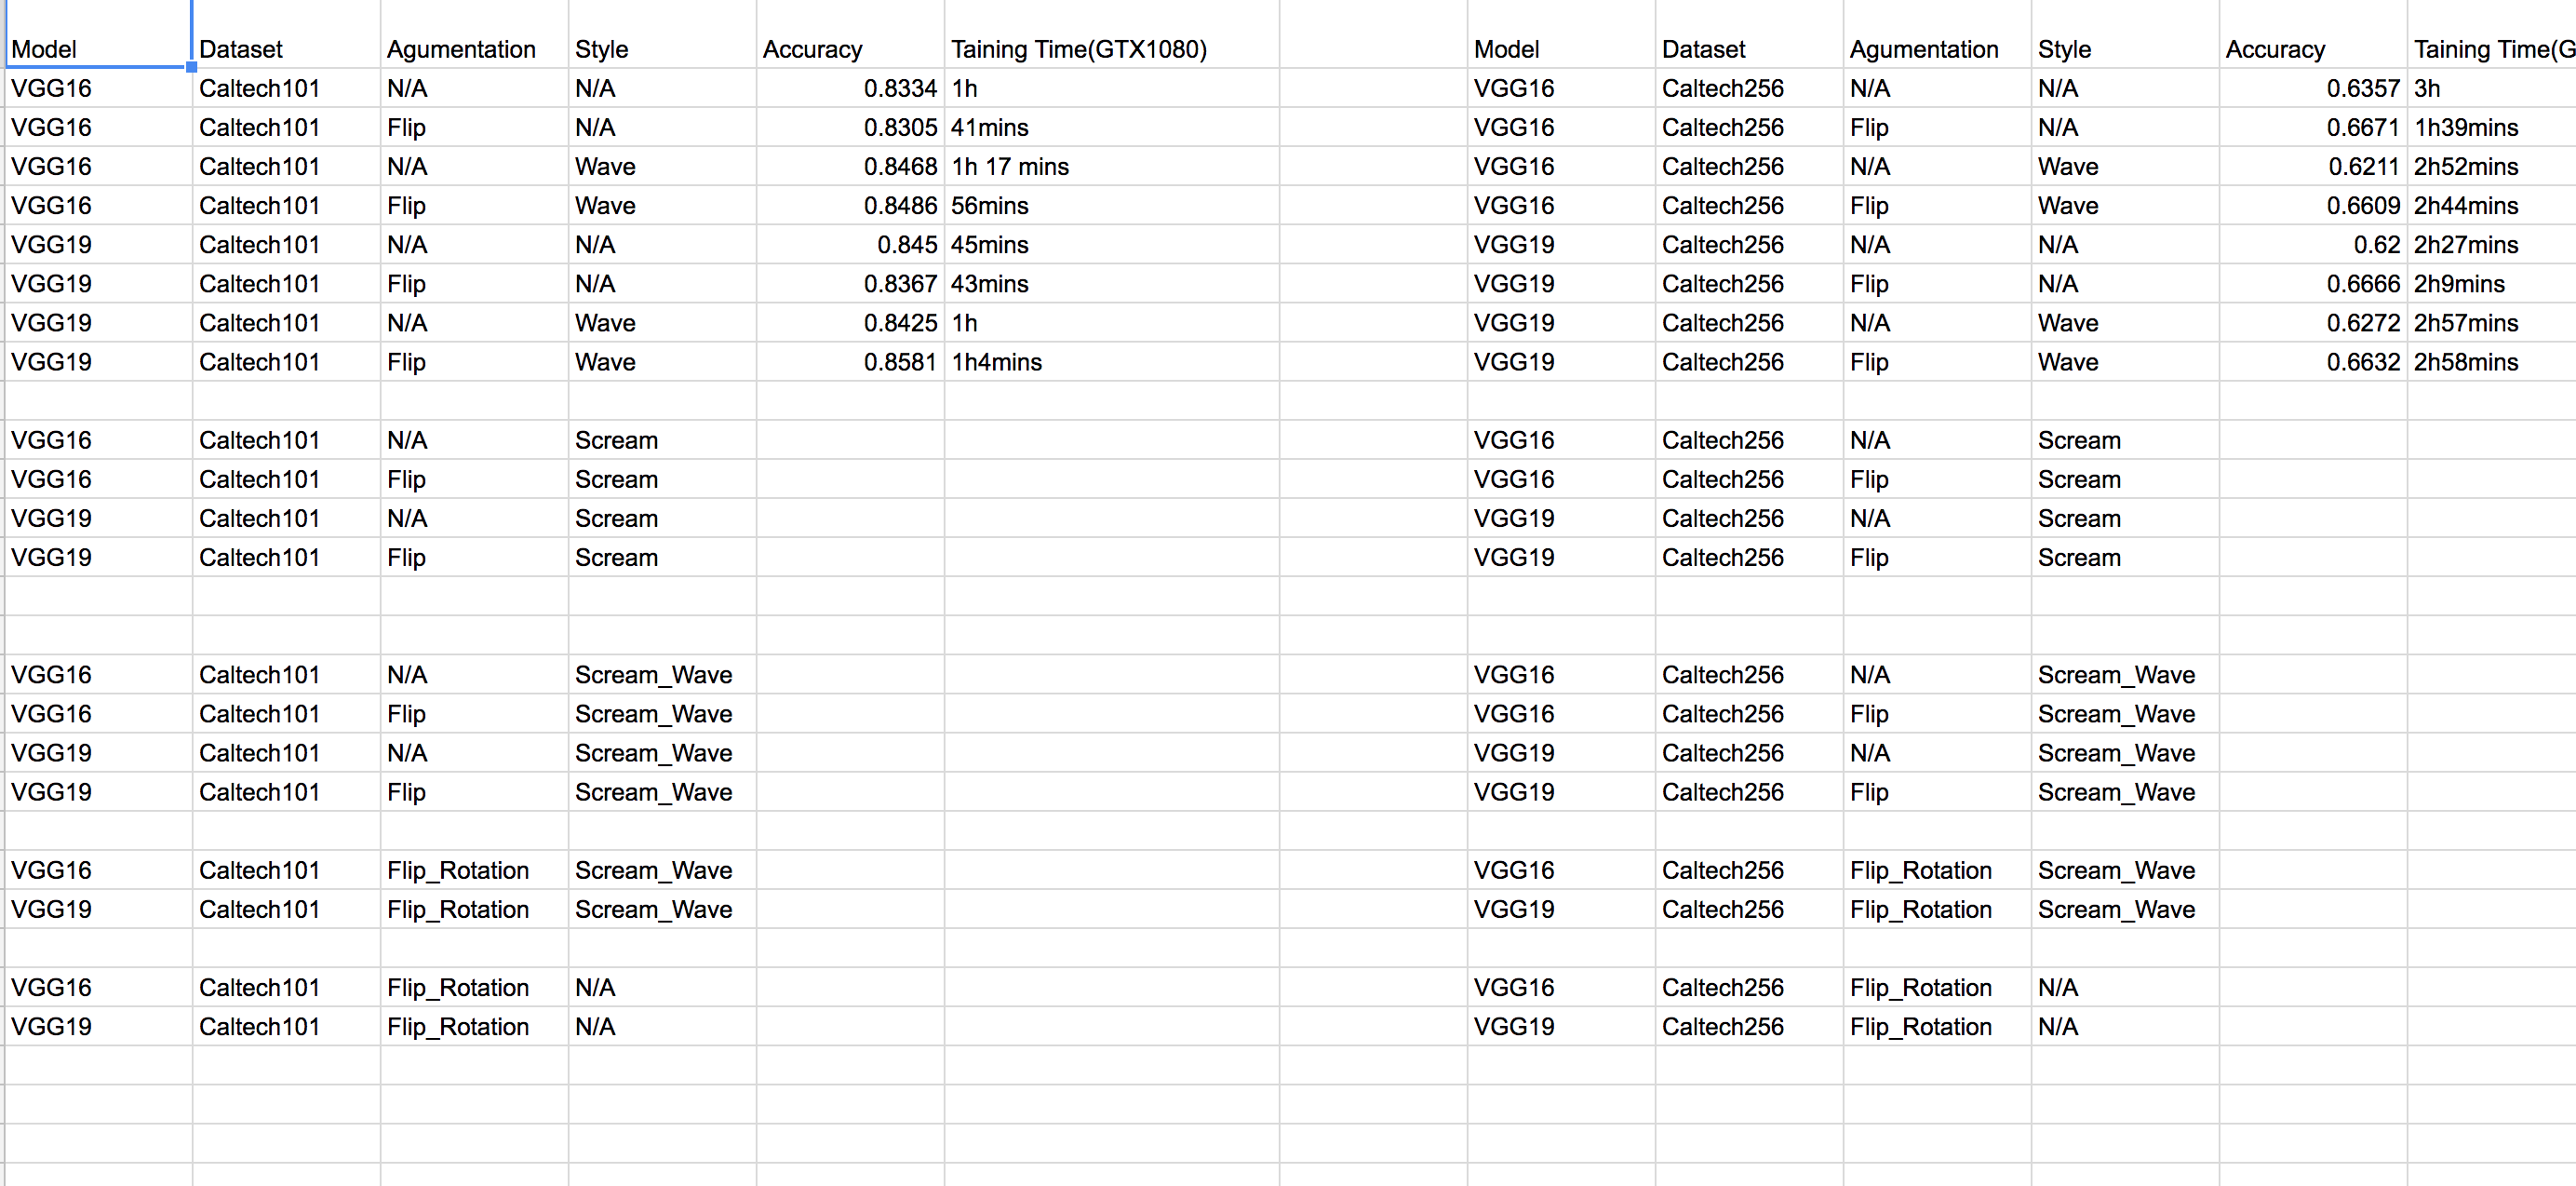
\includegraphics[width=0.4\textwidth, height=0.28\textwidth]{results.png}
\end{center}
\vspace{-20pt}
  \caption{Results.}
  \vspace{-0pt}
\end{wrapfigure}

\section{Conclusion}
Data augmentation has been shown to produce promising ways to increase the accuracy of classification tasks. While traditional augmentation is very effective alone, other techniques enabled by CycleGAN and other similar networks are promising. We experimented with our own way of combining training images allowing a neural net to learn augmentations that best improve the ability to correctly classify images. If given more time, we would like to explore more complex architecture and more varied datasets. To mimic industrial applications, using a VGG16 instead of SmallNet can help us determine if augmentation techniques are still helpful given complex

enough networks that already deal with many overfitting and regularization problems. Finally, although GANs and neural augmentations do not perform much better than traditional augmentations and consume almost 3x the compute time or more, we can always combine data augmentation techniques. Perhaps a combination of traditional augmentation followed by neural augmentation further improves classification strength.

Given the plethora of data, we would expect that such data augmentation techniques might be used to benefit not only classification tasks lacking sufficient data, but also help improve the current state of the art algorithms for classification. Furthermore, the work can be applicable in more generic ways, as ”style” transfer can be used to augment data in situations were the available data set is unbalanced. For example, it would be interesting to see if reinforcement learning techniques could benefit from similar data augmentation approaches. We would also like to explore the applicability of this technique to videos. Specifically, it is a well known challenge to collect video data in different conditions (night, rain, fog) which can be used to train selfdriving vehicles. However, these are the exact situations under which safety is the most critical. Can our style transfer method be applied to daytime videos so we can generate night time driving conditions? Can this improve safety? If such methods are successful, then we can greatly reduce the difficulty of collecting sufficient data and replace them with augmentation techniques, which by comparison are much more simpler.

\bibliographystyle{apalike}

\bibliography{imvip2018}


\end{document}

